% 65-57(65쪽) — 밑변 10, 높이 8 인 이등변삼각형 ABC 와 그 안의 직사각형 DEFG(연한 주황색 채움). 스캔 그림이라 TikZ 로 다시 그림.
% 라벨은 원문 그대로 A·B·C·D·E·F·G·8·10. 직사각형의 가로·세로는 답(넓이가 최대일 때의 둘레)이 읽히지 않게 임의의 위치로 그렸다.
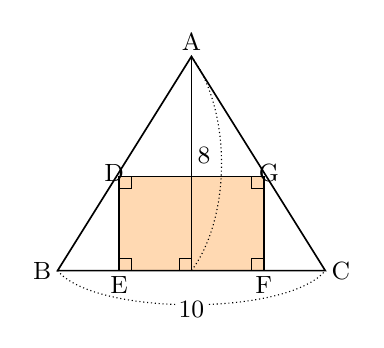
\begin{tikzpicture}[scale=0.34, line width=0.5pt]
  \def\hh{3.52}
  \def\ww{2.7}
  \coordinate (B) at (-5,0);
  \coordinate (C) at (5,0);
  \coordinate (A) at (0,8);
  \coordinate (E) at (-\ww,0);
  \coordinate (F) at (\ww,0);
  \coordinate (D) at (-\ww,\hh);
  \coordinate (G) at (\ww,\hh);
  \fill[orange!30] (D) -- (E) -- (F) -- (G) -- cycle;
  \draw[line width=0.6pt] (A) -- (B) -- (C) -- cycle;
  \draw[line width=0.6pt] (D) -- (E) -- (F) -- (G) -- cycle;
  \draw[line width=0.6pt] (A) -- (0,0);
  % 높이 8 · 밑변 10 을 나타내는 원문의 점선 호
  \draw[densely dotted, line width=0.4pt] (A) .. controls (1.5,6) and (1.5,2) .. (0,0);
  \draw[densely dotted, line width=0.4pt] (B) .. controls (-3.6,-1.7) and (3.6,-1.7) .. (C);
  \node[right, font=\small, inner sep=1.5pt] at (0.05,4.3) {$8$};
  \node[fill=white, font=\small, inner sep=1pt] at (0,-1.45) {$10$};
  % 직각 표시
  \draw[line width=0.4pt] (-\ww+0.45,\hh) -- (-\ww+0.45,\hh-0.45) -- (-\ww,\hh-0.45);
  \draw[line width=0.4pt] (\ww-0.45,\hh) -- (\ww-0.45,\hh-0.45) -- (\ww,\hh-0.45);
  \draw[line width=0.4pt] (-\ww+0.45,0) -- (-\ww+0.45,0.45) -- (-\ww,0.45);
  \draw[line width=0.4pt] (\ww-0.45,0) -- (\ww-0.45,0.45) -- (\ww,0.45);
  \draw[line width=0.4pt] (-0.45,0) -- (-0.45,0.45) -- (0,0.45);
  % 라벨(원문 그대로)
  \node[above, font=\small, inner sep=2pt] at (A) {$\mathrm{A}$};
  \node[left, font=\small, inner sep=2pt] at (B) {$\mathrm{B}$};
  \node[right, font=\small, inner sep=2pt] at (C) {$\mathrm{C}$};
  \node[above left=-3pt, font=\small, inner sep=1pt] at (D) {$\mathrm{D}$};
  \node[above right=-3pt, font=\small, inner sep=1pt] at (G) {$\mathrm{G}$};
  \node[below, font=\small, inner sep=2pt] at (E) {$\mathrm{E}$};
  \node[below, font=\small, inner sep=2pt] at (F) {$\mathrm{F}$};
\end{tikzpicture}
